\begin{frame}
  \frametitle{简介}
  人工生命:研究具有某些生命基本特征的人工系统。包括两方面的内容:
	 \begin{enumerate}
	    \item{研究如何利用计算技术研究生物现象}
	    \item{研究如何利用生物技术研究计算问题}
	  \end{enumerate}
    我们关注的是第二点。已有很多源于生物现象的计算技巧,例如神经网络和遗传算法。现在讨论另一种生物系统---社会系统:由简单个体组成的群落和环境及个体之间的相互行为。
\end{frame}


\begin{frame}
  \frametitle{Nature’s examples of SI(1)}
    \begin{figure}[htbp]
      \centering
      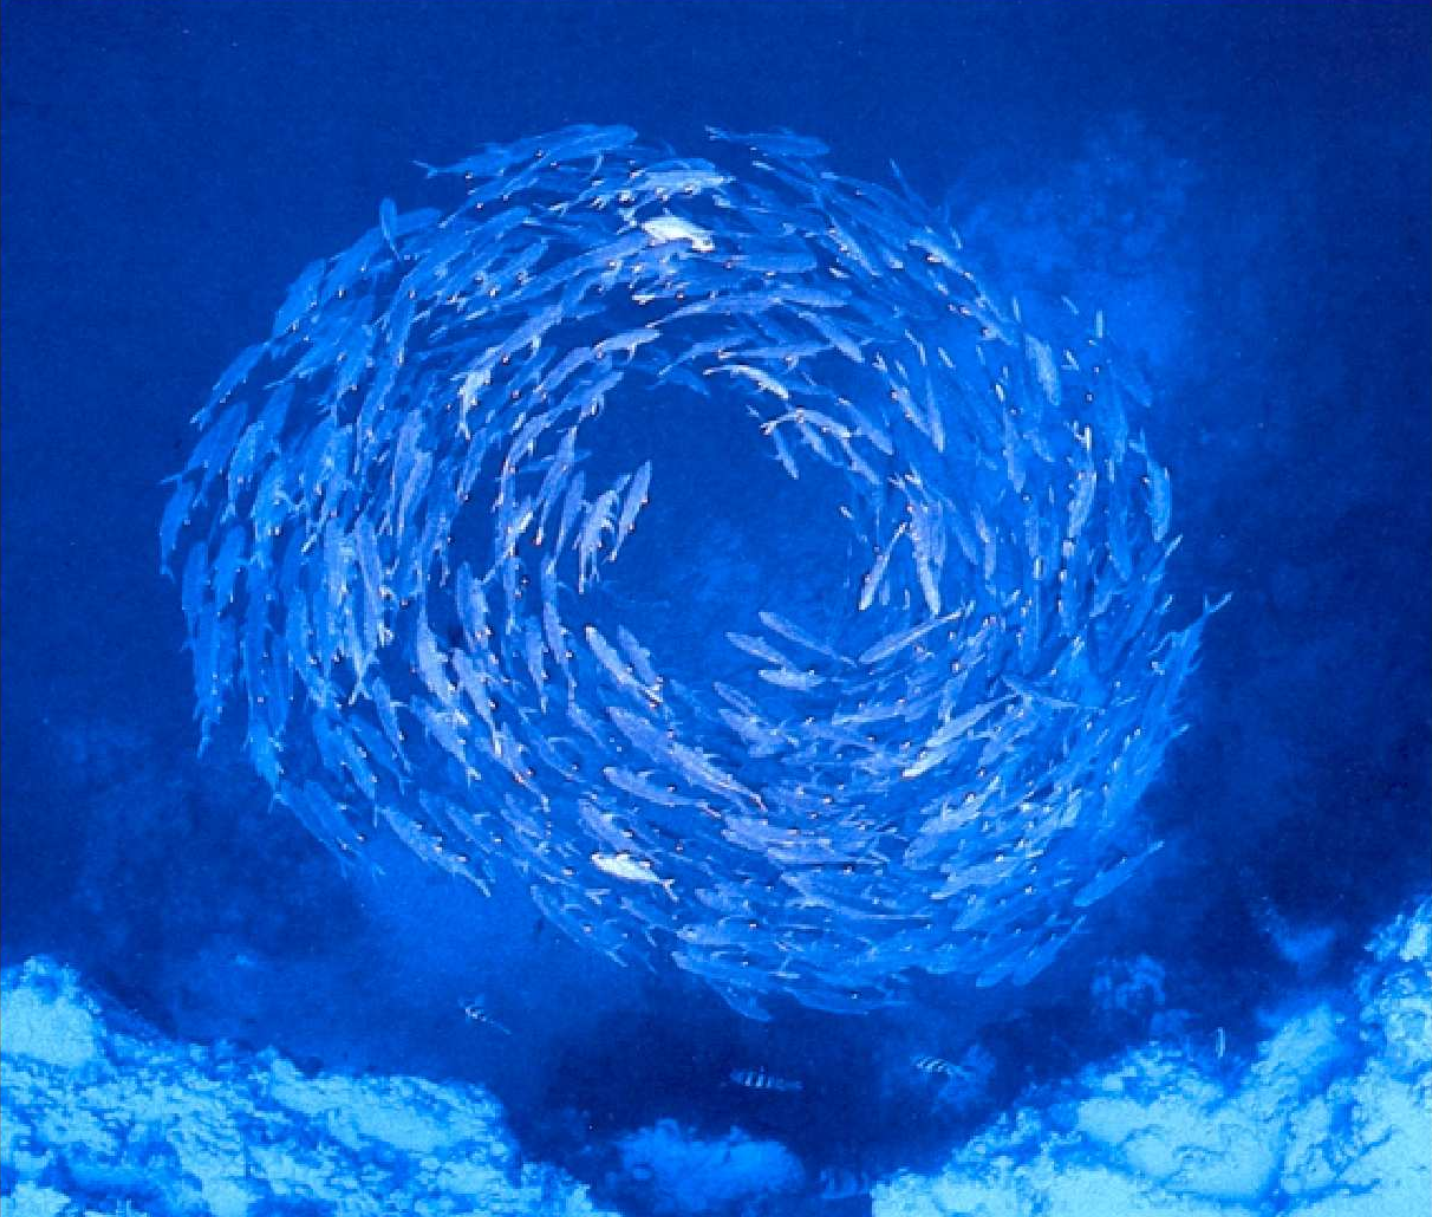
\includegraphics[width=6cm]{pic/si1.png}
      \caption{Fish schooling}
    \end{figure}
\end{frame}

\begin{frame}
  \frametitle{Nature’s examples of SI(2)}
    \begin{figure}[htbp]
      \centering
      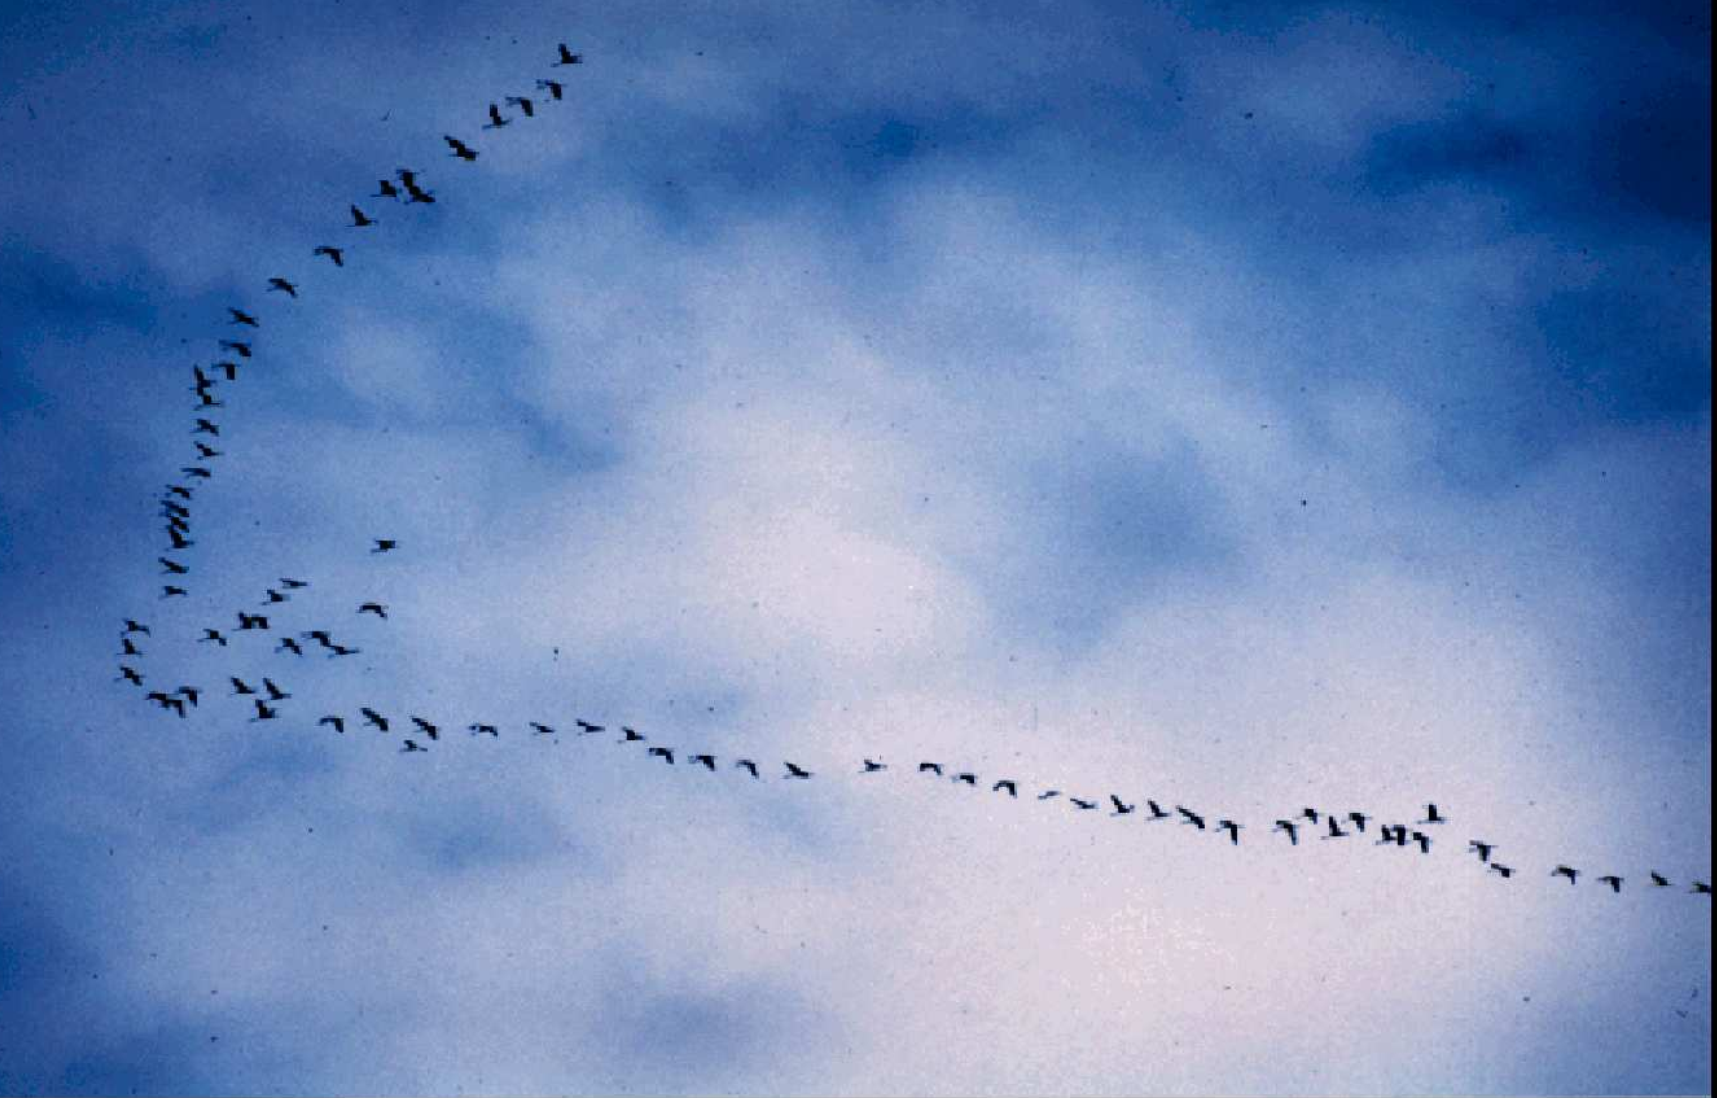
\includegraphics[width=8cm]{pic/si2.png}
      \caption{Birds flocking in V-formation}
    \end{figure}
\end{frame}

\begin{frame}
  \frametitle{Nature’s examples of SI(3)}
    \begin{figure}[htbp]
      \centering
      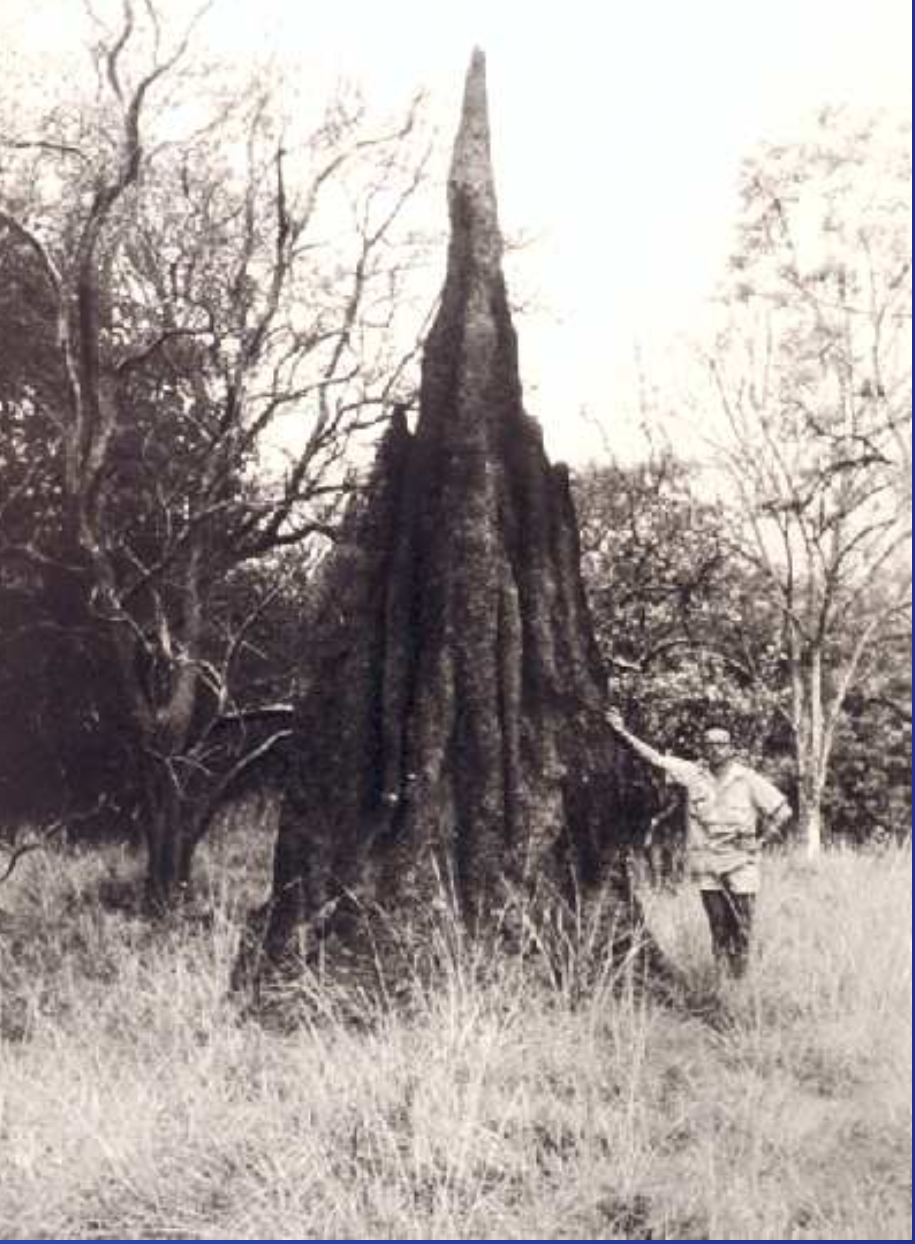
\includegraphics[width=4cm]{pic/si3.png}
      \caption{Termites’ nest}
    \end{figure}
\end{frame}

\begin{frame}
  \frametitle{Nature’s examples of SI(4)}
    \begin{figure}[htbp]
      \centering
      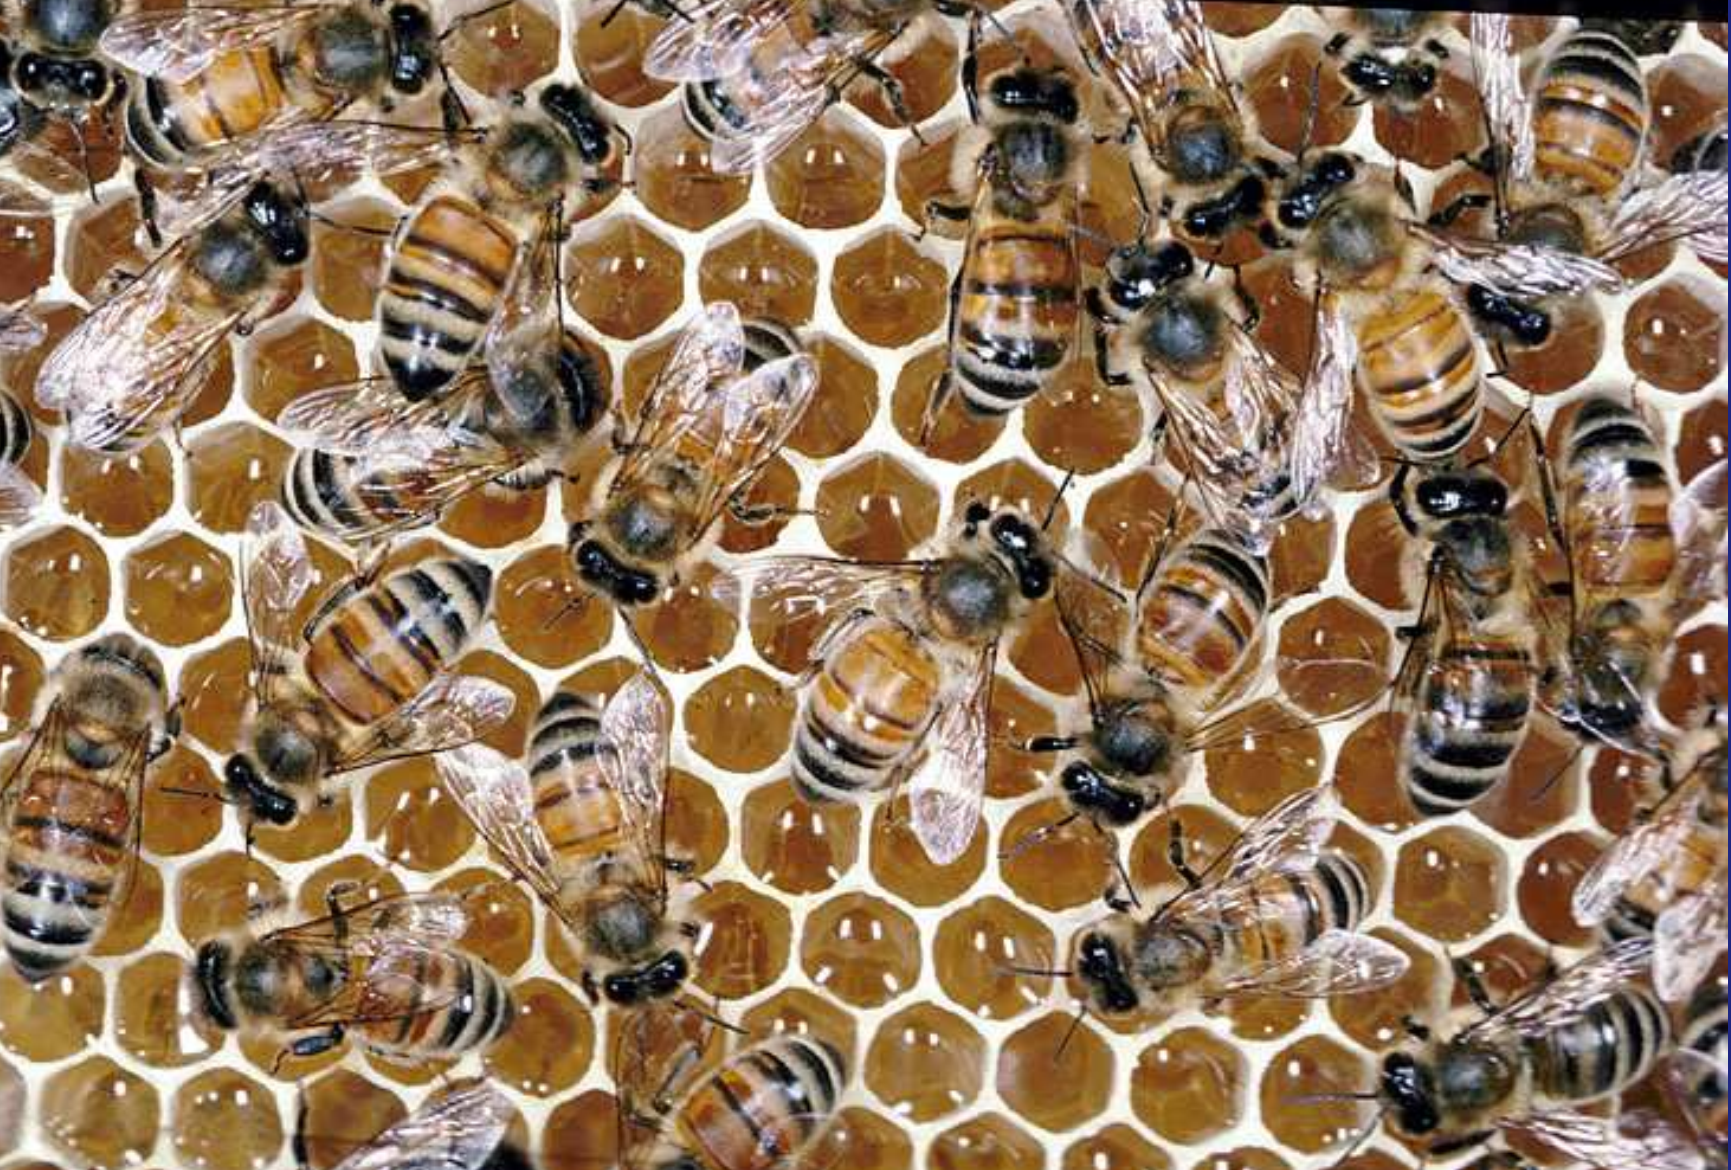
\includegraphics[width=8cm]{pic/si4.png}
      \caption{Bees’ comb}
    \end{figure}
\end{frame}

\begin{frame}
  \frametitle{Nature’s examples of SI(5)}
    \begin{figure}[htbp]
      \centering
      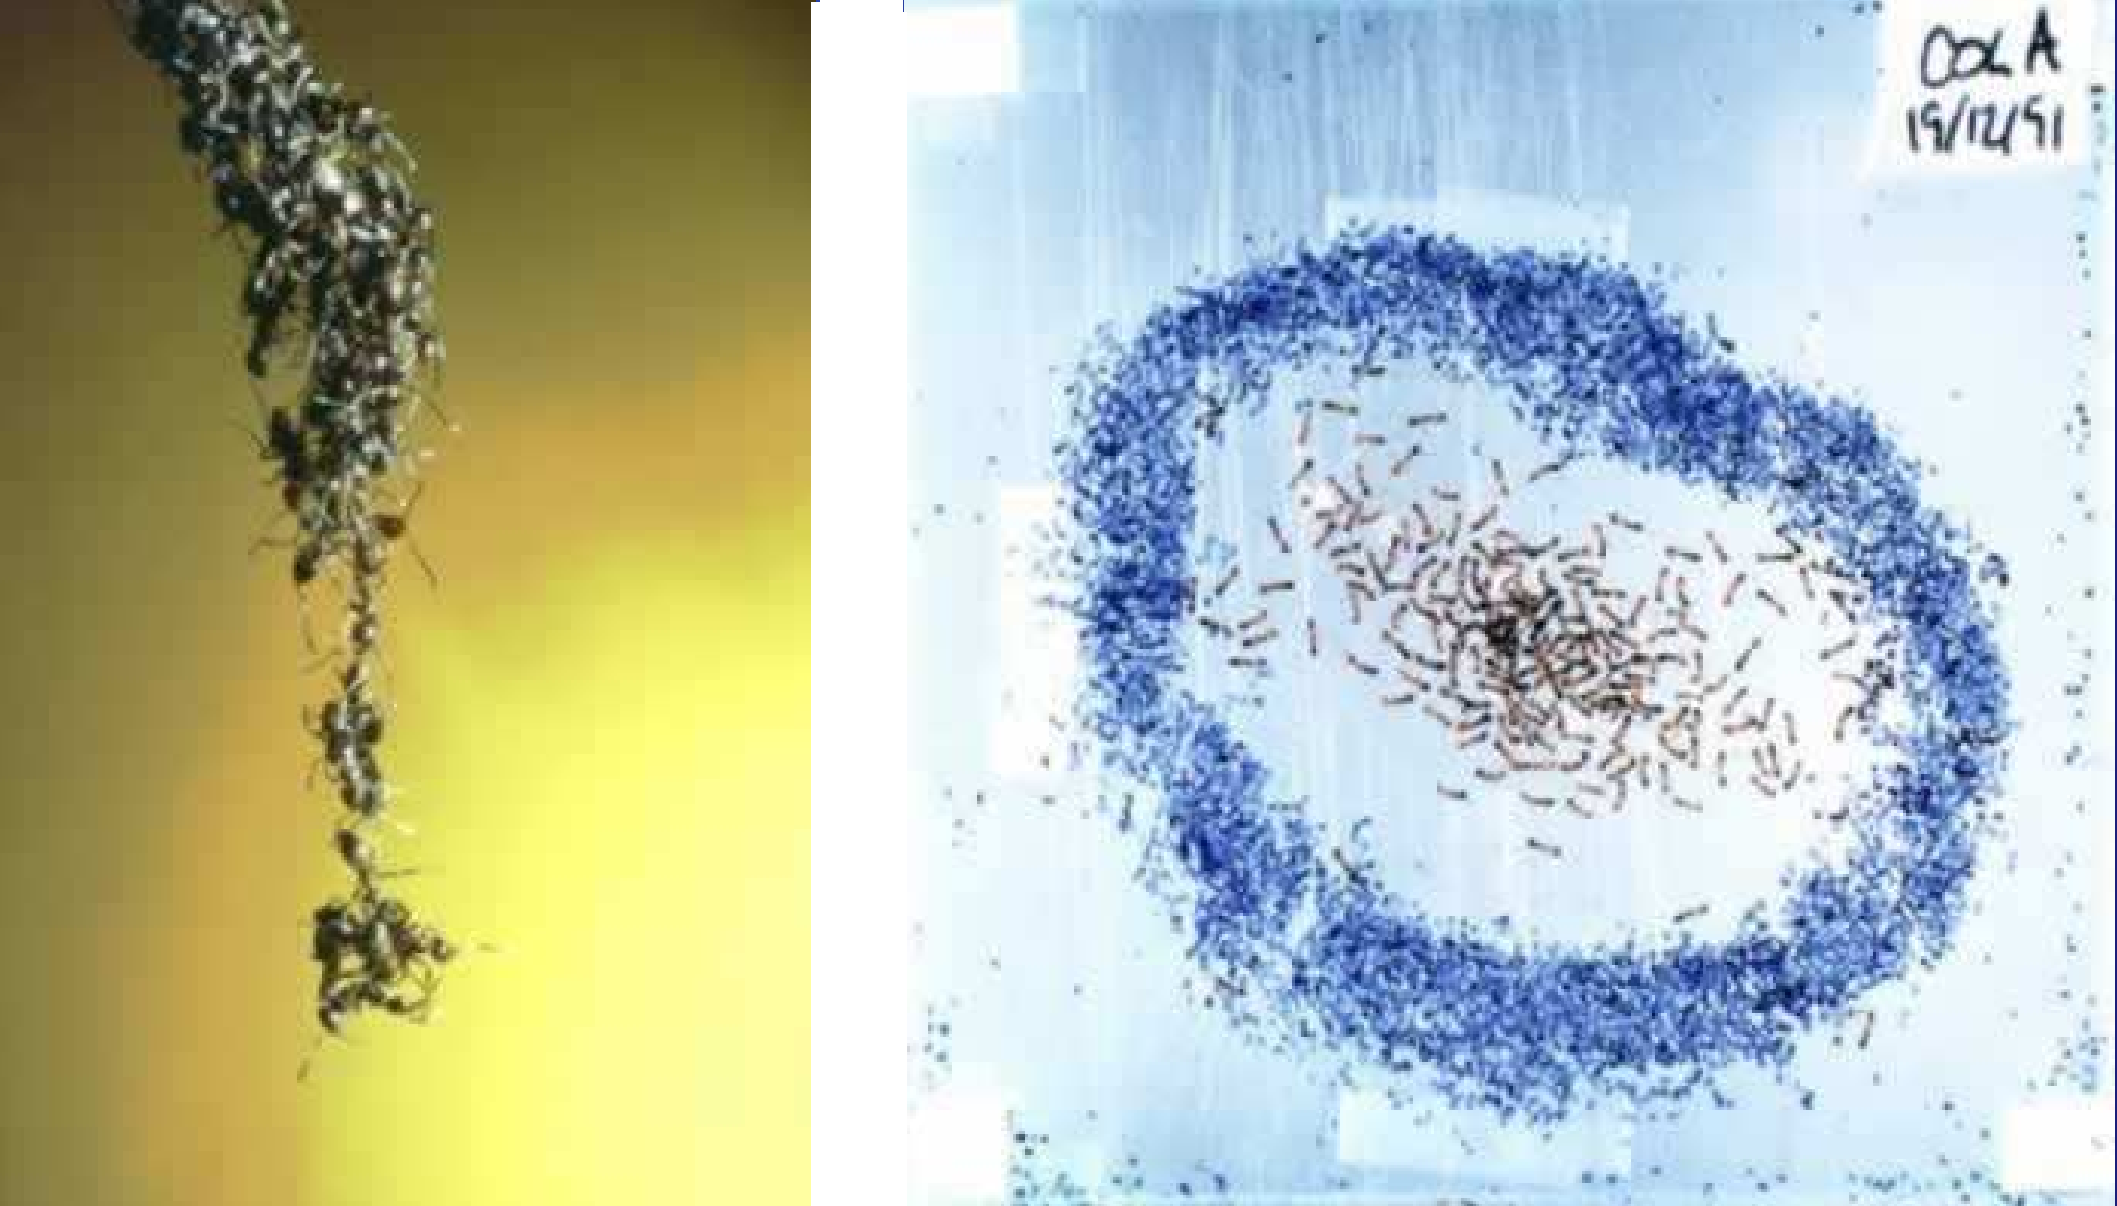
\includegraphics[width=8cm]{pic/si5.png}
      \caption{Ant chain and Ant wall}
    \end{figure}
\end{frame}


\begin{frame}
  \frametitle{群智能}
  $\qquad$模拟系统利用局部信息从而可以产生不可预测的群行为。我们经常能够看到成群的鸟、鱼或者浮游生物。这些生物的聚集行为有利于它们觅食和逃避捕食者。它们的群落动辄以十、百、千甚至万计,并且经常不存在一个统一的指挥者。它们是如何完成聚集、移动这些功能呢?
  \\
  Millonas提出的群体智能的5个原则:
   \begin{enumerate}
      \item{接近性原则:群体应能够实现简单的时空计算}
      \item{优质性原则:群体能够响应环境要素}
      \item{变化相应原则:群体不应把自己的活动限制在一狭小范围}
      \item{稳定性原则:群体不应每次随环境改变自己的模式}
      \item{适应性原则:群体的模式应在计算代价值得的时候改变}
    \end{enumerate}
\end{frame}

\begin{frame}
  \frametitle{对鸟群行为的模拟}
  $\qquad$对鸟群行为的模拟: Reynolds、Heppner和Grenader提出鸟群行为的 模拟。他们发现,鸟群在行进中会突然同步的改变方向,散开或者聚集等。那么一定有某种潜在的能力或规则保证了这些同步的行为。这些科学 家都认为上述行为是基于不可预知的鸟类社会行为中的群体动态学。 在这些早期的模型中仅仅依赖个体间距的操作,也就是说,这中同步是鸟群中个体之间努力保持 最优的距离的结果。
\end{frame}

\begin{frame}
  \frametitle{对鱼群行为的模拟}
  $\qquad$对鱼群行为的研究:生物社会学家E.O.Wilson对鱼群进行了研究。提出:“至少在理论上,鱼群的个体成员能够受益于群体中其他个体在寻找食物的过程中的发现和以前的经验,这种受益超过了个体之间的竞争所带来的利益消耗,不管任何时候食物资源不可预知的分散。”这说明,同种生物之间信息的社会共享能够带来好处。这是PSO的基础。 
\end{frame}